\chapter{Protocolli Automotive} %\label{1cap:spinta_laterale}
% [titolo ridotto se non ci dovesse stare] {titolo completo}
%

\begin{citazione}
In questo capitolo verranno illustrati i dettagli sui principali protocolli utilizzati nel mondo \emph{Automotive}, evidenziando punti di forza e debolezze. Successivamente, verrà effettuato un confronto tra questi in termini di prestazioni, applicabilità, costi, ecc.
\end{citazione}

\section{CAN}

\subsection{Caratteristiche del protocollo}
Il protocollo \emph{CAN} (Controller Area Network) è un protocollo basato su scambio di messaggi che permette a più dispositivi di trasmettere informazioni in maniera affidabile e in logica basata su \textbf{priorità}. Tutti i messaggi (o "\emph{frame}") inviati sono ricevuti da tutti i dispositivi connessi alla rete e, per questa ragione, la tipica topologia di rete usata in sinergia con \emph{CAN} è \textbf{BUS}, ovvero tutti i dispositivi appartenenti alla rete vengono collegati su un singolo cavo detto anche \emph{backbone}. Inoltre, è un protocollo \textbf{multi-master} \cite{huang_2019_invehicle}, in quanto non ha bisogno di un nodo master che fa da arbitro per l'intera rete ma tutti i nodi connessi sono in grado di comunicare autogestendosi, utilizzando come schema di arbitraggio \textbf{CSMA/CD} (Carrier-Sense Multiple Access with Collision Detection) \cite{can_notes}. Con questo schema, un dispositivo che vuole trasmettere un messaggio si mette prima in ascolto sul cavo e, se non rileva trasmissioni in corso, comincia a trasmettere il messaggio ascoltando quello che sta inviando. Se nel mentre che sta inviando il messaggio rileva un'interferenza, generata dall'arrivo di un altro messaggio già in fase di trasmissione, ferma immediatamente la trasmissione, trasmette una sequenza di \textbf{jamming} con lo scopo di avvertire gli altri dispositivi che è avvenuta una collisione e attende un tempo casuale prima di ritrasmettere (ovviamente dopo aver stabilito che il canale è libero) \cite{wikipedia_csmacd}. Uno schema per comprendere meglio il funzionamento dell'algoritmo \textbf{CSMA/CD} è mostrato nella Figura \ref{fig:csmacd-scheme}.
\begin{figure}[h]
    \centering
    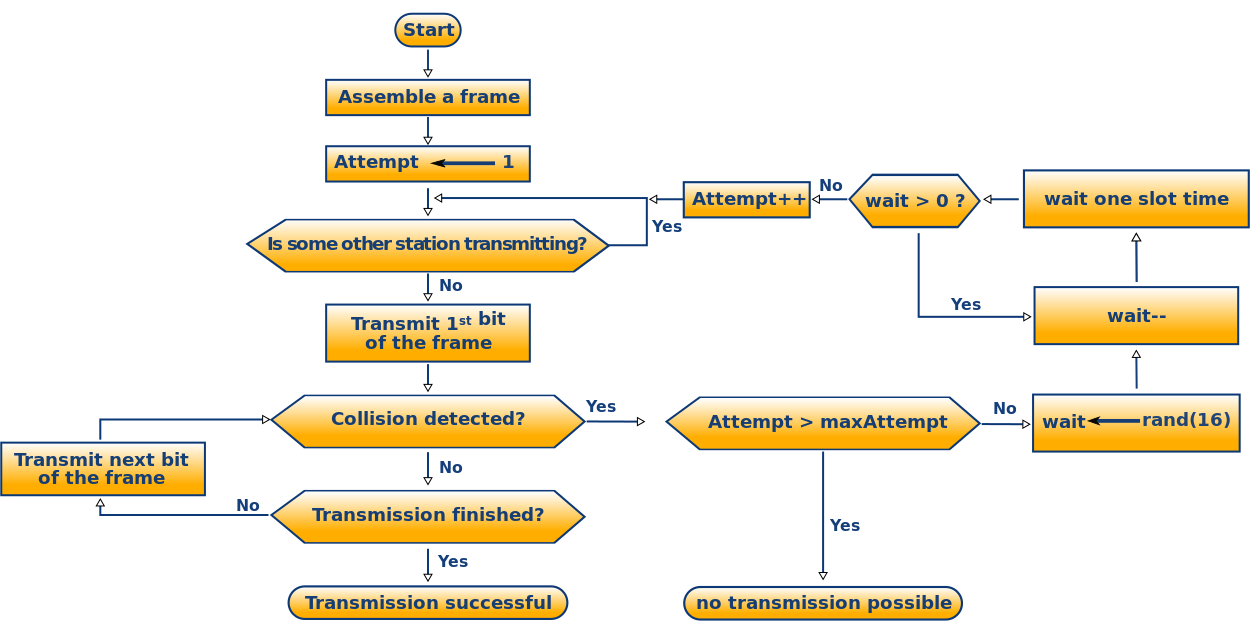
\includegraphics[width=0.7\textwidth]{capitoli/figure-protocolli/CSMACD-Algorithm.png}
    \caption{Diagramma di flusso di un algoritmo \textbf{CSMA/CD} con ritrasmissione}
    \label{fig:csmacd-scheme}
\end{figure}

Ogni dispositivo connesso alla rete viene chiamato \textbf{nodo} e deve essere composto almeno da una \emph{CPU} (processore per far funzionare tutto il dispositivo), un controller \emph{CAN} (componente che sappia parlare il protocollo \emph{CAN}) e un \emph{ricetrasmettitore} (componente che "legge e scrive" sui cavi elettrici).\\
È il protocollo più uitlizzato in ambito \emph{Automotive} in quanto il suo utilizzo ha i seguenti vantaggi:

\begin{itemize}
    \item È un protocollo che richiede un cablaggio semplicissimo e poco costoso (un semplice cavo con due fili), riducendo la latenza, il peso della rete (in termini di kilogrammi), il numero di cavi necessari e il numero di errori;
    \item È completamente centralizzato e, per questa ragione, basta un qualunque punto di aggancio alla rete per accedere a tutto il traffico in circolazione e comunicare con tutte le \emph{ECU} connesse. Questo semplifica di molto il logging delle informazioni per fini diagnostici e la configurazione delle centraline;
    \item È molto robusto contro interferenze elettromagnetiche e disturbi elettrici, rendendolo ideale per applicazioni \textbf{safety-critical};
    \item Grazie all'integrazione di una logica basata su \textbf{priorità}, messaggi con \emph{ID} associati ad una priorità alta sono i primi ad accedere alla rete, senza causare interruzioni agli altri messaggi;
    \item Eliminando kilometri di cavi elettrici in eccesso, permette di ridurre il peso totale dell'automobile su cui è installata la rete migliorando anche i consumi di carburante;
    \item Dal momento che i chip e la strumentazione necessaria è molto semplice ed economica, abbassando di molto il costo necessario alla creazione della rete e delle \emph{ECU};
    \item Prevede meccanismi di correzione e rilevazione degli errori molto efficaci, permettendo alle informazioni di arrivare integre a destinazione;
    \item È facile aggiungere o rimuovere nodi dalla rete. \cite{can_bus_dewesoft}
\end{itemize}

\begin{figure}[h]
    \begin{subfigure}{0.45\textwidth}
        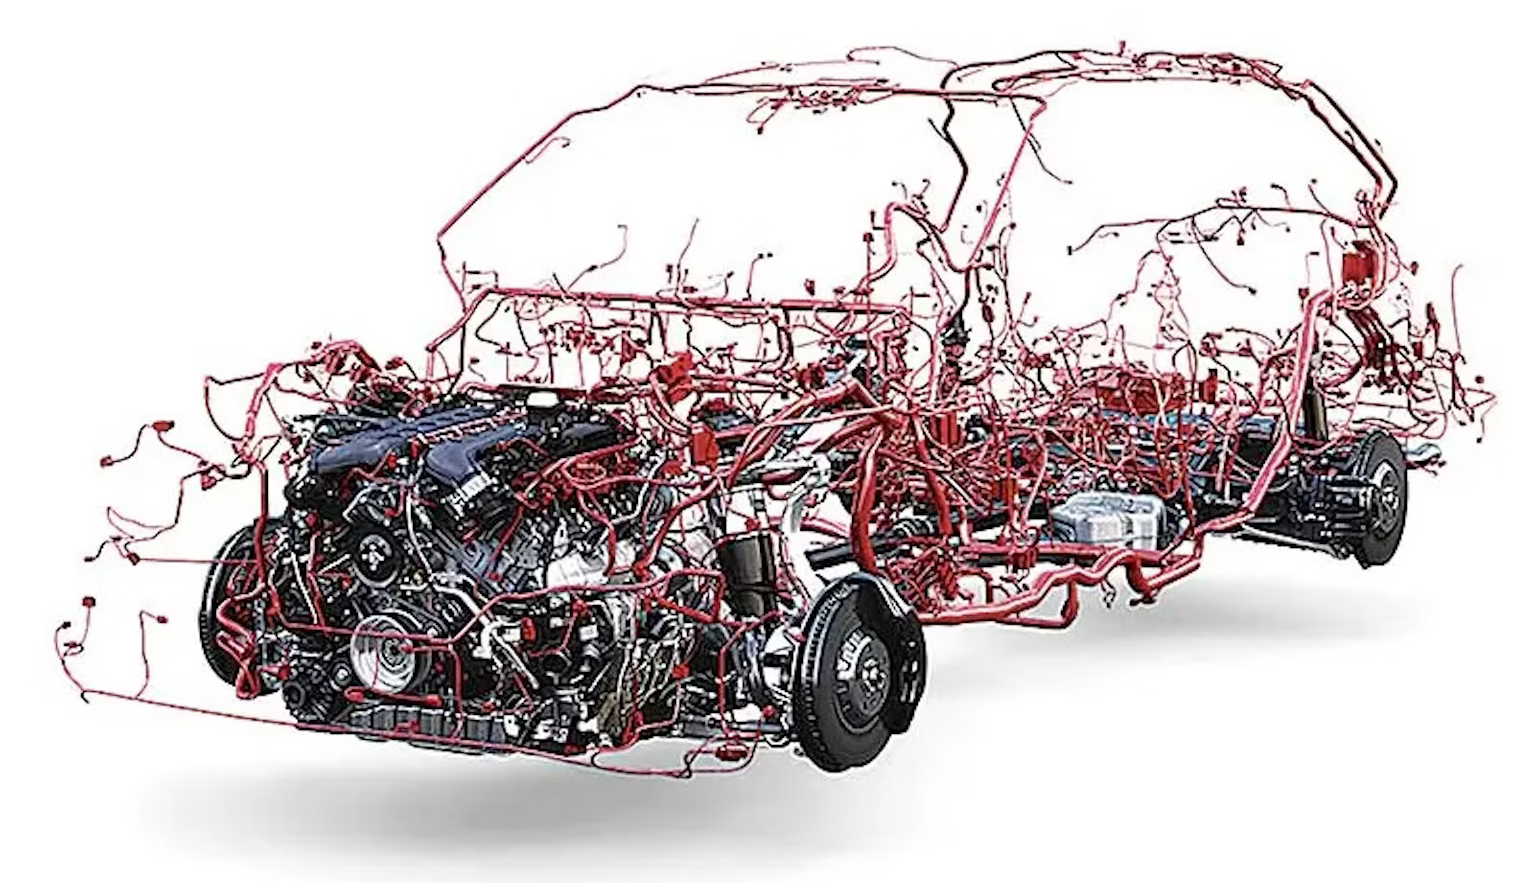
\includegraphics[width=1\textwidth]{capitoli/figure-protocolli/electrical-wiring-no-can.png}
        \caption{Cablaggio tipico di un'automobile che \textbf{NON} utilizza \emph{CAN}}
        \label{fig:electrical-wiring-no-can}
    \end{subfigure}
    \hfill
    \begin{subfigure}{0.45\textwidth}
        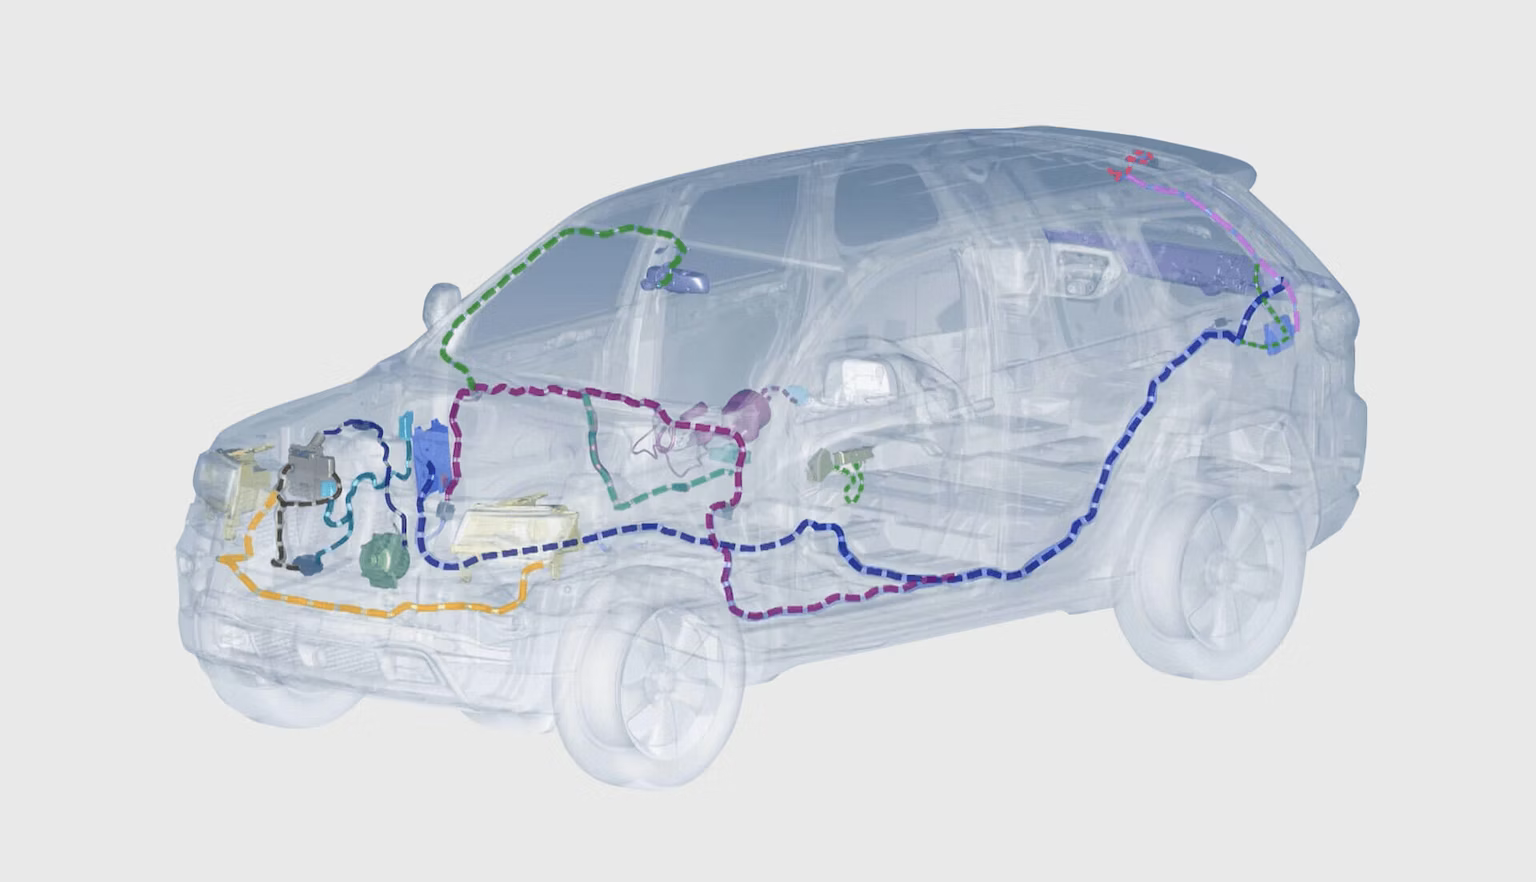
\includegraphics[width=1\textwidth]{capitoli/figure-protocolli/electrical-wiring-can.png}
        \caption{Cablaggio tipico di un'automobile che utilizza \emph{CAN}}
        \label{fig:electrical-wiring-can}
    \end{subfigure}
    \caption{Differenza di cablaggi con e senza \emph{CAN}}
    \label{fig:electrical-wiring-differences}
\end{figure}

Per via dei motivi sopracitati, oltre ad essere il protocollo più utilizzato in campo \emph{Automotive} è anche utilizzato in moltissimi altri ambiti, tra cui:

\begin{itemize}
    \item Aeronautica;
    \item Ascensori ed elevatori;
    \item Industrie e fabbriche;
    \item Navi;
    \item Elettrodomestici casalinghi come lavatrici, asciugatrici, ecc. \cite{can_bus_dewesoft}
\end{itemize}

\subsection{Struttura dei messaggi}
Ogni messaggio \emph{CAN} ha una struttura ben definita ed è composto da \textbf{header}, \textbf{payload} e \textbf{trailer}. Inoltre, è possibile individuare due tipologie di messaggi che sono \textbf{standard} e \textbf{esteso}, la cui unica vera differenza sta nella presenza di un campo \emph{ID} aggiuntivo nel messaggio (quindi cambia solo la lunghezza complessiva del messaggio).

\begin{figure}[h]
    \centering
    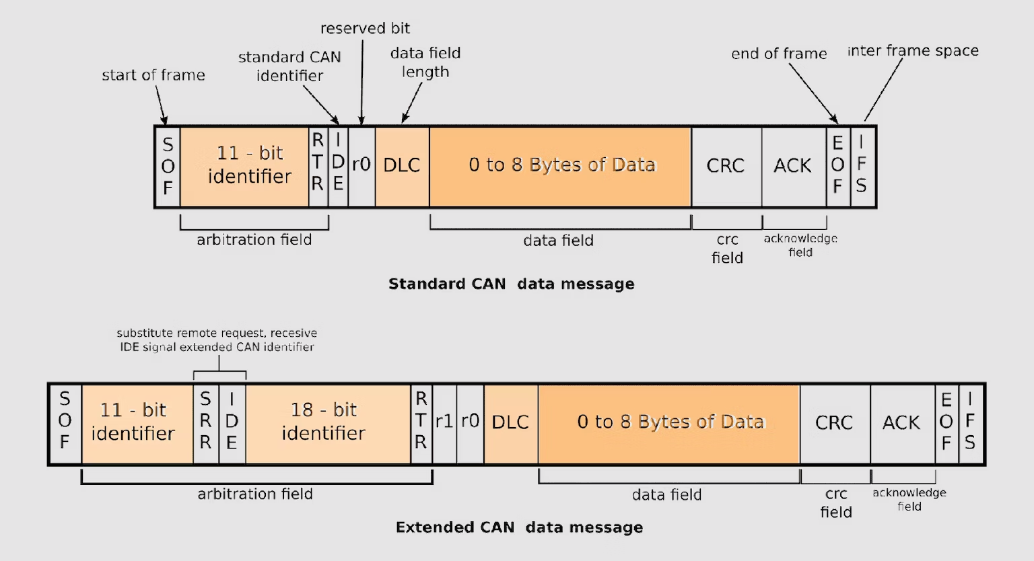
\includegraphics[width=0.7\textwidth]{capitoli/figure-protocolli/can-data-message-structure.png}
    \caption{Struttura dei messaggi \emph{CAN} \textbf{standard} ed \textbf{estesi}}
    \label{fig:can-message-structure}
\end{figure}

I vari campi di un tipico messaggio \emph{CAN} \textbf{standard} sono:
\begin{itemize}
    \item \textbf{SOF} (Start of Frame): 1 bit che indica l'inizio del messaggio e sincronizza i nodi dopo un periodo di inattività;
    \item \textbf{ID}: 11 bit che definiscono la priorità del messaggio, dove un identificativo più basso corrisponde ad una priorità più alta;
    \item \textbf{RTR}: 1 bit che viene impostato a $0$ (o \emph{dominante}) quando quello che si sta inviando è una \textbf{richiesta di informazione} (non un'informazione) e $1$ (o \emph{recessivo}) in caso contrario. Quando il bit viene impostato a $0$, non viene inviato nessun dato e l'\textbf{ID} determina l'informazione richiesta (quindi il nodo \emph{target});
    \item \textbf{IDE} (Identifier Extension): 1 bit che determina se il pacchetto è standard ($0$) o esteso ($1$);
    \item \textbf{r0}: 1 bit riservato che è privo di significato e lasciato per eventuali sviluppi futuri. Di solito è lasciato a $0$, ma anche se impostato a $1$ non fa differenza e viene accettato lo stesso;
    \item \textbf{DLC} (Data Length Code): 4 bit che indicano la lunghezza in \textbf{byte} del payload che contiene il messaggio;
    \item \textbf{Data}: 64 bit che indicano il dato che si sta inviando con il messaggio;
    \item \textbf{CRC} (Cyclic Redundancy Check): 16 bit che indicano il \textbf{checksum}, ovvero una \emph{somma} associata al campo \textbf{data} che viene utlizzata, tramite particolari operazioni matematiche, per effettuare rilevamento degli errori;
    \item \textbf{ACK} (ACKnowledgment): 1 bit che determina se un messaggio è stato ricevuto con successo ($0$) oppure sono stati rilevati degli errori ($1$). Chi invia il messaggio imposta il bit a $1$, metre chi riceve con successo imposta il bit a $0$;
    \item \textbf{EOF} (End of Frame): 7 bit che denotano la fine di un messaggio \emph{CAN}.
    \item \textbf{IFS} (Inter Frame Space): 3 bit recessivi (impostati a $1$) che separano il messaggio appena trasmesso da un nuovo messaggio. Dopo i primi 3 bit a $1$, il primo bit dominante (impostato a $0$) rilevato corrisponderà ad un bit \textbf{SOF}. \cite{can_bus_dewesoft} \cite{wikipedia_canbus}
\end{itemize}

Oltre ai campi di un messaggio \emph{standard}, i campi aggiuntivi in un messaggio \textbf{esteso} sono i seguenti:
\begin{itemize}
    \item \textbf{SRR} (Substitute Remote Request): 1 bit impostato a $1$ che serve a far prevalere sempre i messaggi \emph{standard} durante l'arbitraggio;
    \item \textbf{ID}: 18 bit che si aggiungono al primo campo \textbf{ID}, componendo un identificativo di 29 bit totali;
    \item \textbf{R1}: 1 bit riservato come \textbf{R0}, quindi anche in questo caso il valore associato a questo campo non ha significato e viene accettato qualunque sia.
\end{itemize}

Un'altra piccola differenza è che il campo \textbf{IDE} è posizionato prima del bit \textbf{RTR} e, in mezzo a questi due campi è posizionato il secondo campo \textbf{ID}.

\subsection{Tipologie di messaggi}
Il protocollo \emph{CAN} prevede quattro tipologie di messaggi (o \emph{frame}), che si distinguono in base al compito che devono svolgere.
\subsubsection{Data Frames}
Questa tipologia di frame è l'unica che prevede l'utilizzo del campo \textbf{Data} e un \textbf{DLC} diverso da 0. È, quindi, la tipologia di messaggio che un nodo invia per condividere informazioni con uno o più nodi, associando all'identificativo il tipo di dato inviato e la priorità.

\subsubsection{Remote Frames}
Questa tipologia di frame permette ad un nodo di richiedere una specifica informazione
\subsubsection{Error Frames}
\subsubsection{Overload Frames}

\subsection{Varianti del protocollo}

\subsubsection{Low Speed CAN}

\subsubsection{High Speed CAN}

\subsubsection{CAN FD}

\section{FlexRay}

\section{LIN}

\section{Confronto tra i tre protocolli}

\newpage
